\scanpage{11}
\[
 \unsure{=|\Rightarrow}
\]
\[
 \begin{aligned}
 &\mathbb P\left(
 \begin{tikzpicture}[x=.0043cm,y=-.0043cm,baseline={(0,82)},line cap=round,line join=round]
 \draw[line width=.5pt] (18,12) -- (59,76) (64,1) -- (23,78);
 \draw[line width=.5pt] (0,1) -- (30,3) (63,0) -- (76,1)
 (0,80) -- (26,78) (58,76) -- (78,77);
 \end{tikzpicture}\right)\qquad
 P(X\times\unsure{Z|2})\overset{?}{\simeq}
 \operatorname{Hom}(\deleted{\unsure{\mathcal E|e}}Z\times X,\mathscr E)\\
 &\hspace{6em}\mathrel{/\!/}\ 
 \overset{\unsure{\deleted{M}|M|\deleted{U}|U}\quad\deleted{H}\quad\unsure{\deleted{R}|R}}
 {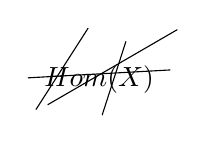
\begin{tikzpicture}[baseline=(old.base),line cap=round,line join=round]
 \node[inner sep=0pt] (old) at (0,0) {$\rlap{$\operatorname{Hom}(X)$}\phantom{\deleted{\operatorname{Hom}(X)}}$};
 \draw (-.9,.02) -- (.9,.12);
 \draw (-.8,-.38) -- (-.14,.65);
 \draw (.04,-.45) -- (.34,.48);
 \draw (-.65,-.32) -- (.99,.63);
 \end{tikzpicture}}
 \\[-.2em]
 &\hspace{9em}\unsure{\operatorname{Hom}}(X,\underline{\operatorname{Hom}}(\mathscr E,Z)\\
 \unsure{O|0}\subset\mathbb P(X)&\qquad
 \operatorname{Hom}(\mathscr E,\underline{\operatorname{Hom}}(X,Z))\\
 &\qquad\mathrel{/\!/}\\
 &\qquad P(\operatorname{Hom}(X,Z)
 \end{aligned}
\]
% The upper-left X is drawn to retain its detached upper-left serif.
% Raised M/U and R have uncertain cancellation status; no writing chronology is supplied.
% crop-candidate: scan 11
\figure{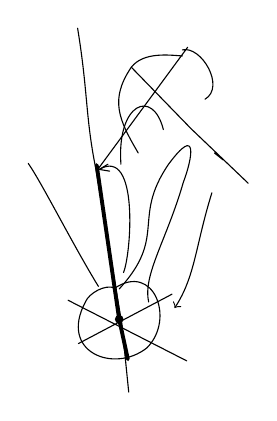
\begin{tikzpicture}[x=.011cm,y=-.011cm,line cap=round,line join=round]
\draw (63,1) .. controls (75,74) and (72,104) .. (84,163) -- (114,342) -- (122,421);
\draw[line width=1.4pt] (85,159) -- (111,337) -- (121,383);
\draw (6,157) .. controls (22,180) and (57,250) .. (87,299);
\draw (64,365) -- (172,308) (52,315) -- (189,385);
\draw (106,301) .. controls (151,271) and (176,337) .. (143,370)
 .. controls (105,400) and (41,375) .. (72,317) .. controls (76,307) and (95,296) .. (106,301);
\fill (111,337) circle (5);
\draw (87,163) -- (190,23) (184,26) .. controls (206,21) and (234,69) .. (210,83)
 (125,46) -- (194,117) -- (260,180) (231,153) -- (221,145);
\draw (133,145) .. controls (110,106) and (100,83) .. (125,46) .. controls (139,28) and (169,32) .. (184,33);
\draw (113,158) .. controls (108,87) and (150,70) .. (162,118);
\draw (88,164) .. controls (134,137) and (125,261) .. (116,283);
\draw (111,302) .. controls (167,241) and (125,221) .. (168,158)
 .. controls (202,112) and (196,150) .. (185,179) .. controls (166,245) and (138,286) .. (145,317);
\draw[->] (218,191) .. controls (199,252) and (199,287) .. (175,324);
\draw (88,164) -- (98,158) (88,164) -- (100,166);
\end{tikzpicture}}
\[
 \begin{aligned}
 \underline{\operatorname{Hom}}(X,Y)&\subset P(X\times Y)\\
 \operatorname{Hom}\left(
 \overset{\unsure{\begin{tikzpicture}[x=.013cm,y=-.013cm,baseline=0,line cap=round,line join=round]
 \draw (0,4) -- (4,1) -- (7,4) -- (12,1) -- (18,3);
 \fill (22,3) circle (1.1); \fill[gray] (28,3) circle (.8);
 \end{tikzpicture}}}{\deleted{\unsure{t|1}}Z}
 \times X,Y\right)&\subset P(Z\times X\times Y)
 \end{aligned}
\]
% Detached wavy trace and spots above the overwritten Z: shape retained, role and hand undetermined.
\diagram{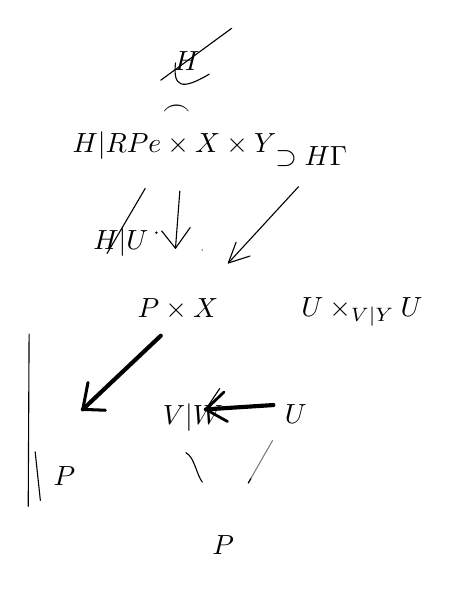
\begin{tikzpicture}[x=.011cm,y=-.011cm,line cap=round,line join=round]
% The diagram is positioned from the observed page, including its short unattached lower strokes.
\node[anchor=base] at (200,59) {$\rlap{$H$}\phantom{\deleted{H}}$};
\draw (170,70) -- (252,10);
\draw (187,50) .. controls (184,78) and (194,82) .. (226,63);
\node[anchor=base] at (188,111) {$\frown$};
\node[anchor=base west] at (57,154) {$\deleted{\unsure{H|R}}P\deleted{\unsure{e}}\times X\times Y$};
\node[anchor=base west] at (291,169) {$\supset\deleted{H}\Gamma$};
\node[anchor=base] at (124,266) {$\rlap{$\unsure{H|U}$}\phantom{\deleted{\unsure{H|U}}}$};
\draw (108,270) -- (152,195);
\draw (192,198) -- (187,264);
\draw (171,244) -- (187,264) -- (204,240);
\fill (165,246) circle (1.5);
\fill[gray] (218,266) circle (1.0);
\draw (329,193) -- (248,281);
\draw (257,257) -- (248,281) -- (273,273);
\node[anchor=base west] at (132,344) {$P\times X$};
\node[anchor=base west] at (321,343) {$U\times_{\unsure{V|Y}}U$};
\draw[line width=1.5pt] (170,365) -- (80,450);
\draw[line width=1.1pt] (86,419) -- (80,450) -- (106,451);
\draw (18,363) -- (17,562);
\draw (25,499) -- (31,555);
\node[anchor=base west] at (35,538) {$P$};
\node[anchor=base] at (207,468) {$\unsure{V|W}$};
\node[anchor=base] at (326,466) {$U$};
\draw[line width=1.5pt] (300,445) -- (222,450);
\draw[line width=1pt] (243,430) -- (222,450) -- (247,464);
\draw (238,426) -- (222,450);
\draw (199,500) .. controls (209,505) and (211,525) .. (218,534);
\draw[gray] (299,486) -- (271,535);
\draw (274,530) -- (271,535);
\node[anchor=base] at (242,618) {$P$};
\end{tikzpicture}}
% crop-candidate: scan 11
\figure{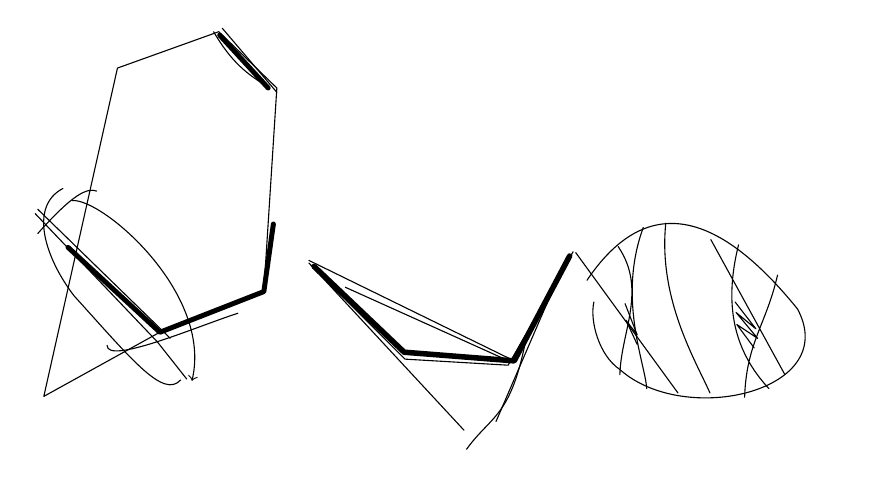
\begin{tikzpicture}[x=.011cm,y=-.011cm,line join=round,line cap=round]
\draw (13,425) -- (98,46) -- (215,4) -- (282,69) -- (267,303) -- (145,352) -- cycle;
\draw[line width=1.8pt] (216,8) -- (272,69) (278,226) -- (267,304) -- (147,351) -- (41,253);
\draw (209,4) .. controls (230,40) and (248,53) .. (272,68) (282,74) -- (219,0);
\draw (6,237) .. controls (47,191) and (63,184) .. (74,188)
 (3,214) -- (144,362) -- (178,405) (6,209) -- (159,358);
\draw (35,185) .. controls (-5,206) and (15,266) .. (48,309)
 .. controls (115,383) and (151,428) .. (171,406);
\draw[->] (46,199) .. controls (80,196) and (208,305) .. (184,407);
\draw (86,366) .. controls (86,389) and (188,345) .. (237,329);
\draw (319,271) -- (430,382) -- (549,389) -- (624,258) (319,271) -- (498,464) (535,454) -- (617,264);
\draw[line width=2pt] (325,275) -- (429,374) -- (556,384) -- (620,263);
\draw (319,268) -- (556,384) (361,299) -- (543,381);
\draw (501,486) .. controls (530,446) and (552,450) .. (570,357);
\draw (627,259) -- (745,421);
\draw (640,291) .. controls (722,169) and (814,239) .. (883,324)
 .. controls (934,419) and (753,461) .. (678,394) .. controls (654,378) and (643,338) .. (648,316);
\draw (676,252) .. controls (710,302) and (679,351) .. (678,400)
 (705,230) .. controls (675,312) and (707,386) .. (709,416)
 (731,225) .. controls (722,312) and (765,383) .. (782,421);
\draw (783,244) -- (868,399) (815,250) .. controls (797,322) and (811,374) .. (850,416)
 (860,285) .. controls (847,342) and (824,363) .. (822,426);
\draw (684,318) -- (698,354) -- (685,337) -- (698,365)
 (811,316) -- (835,347) -- (812,328) -- (837,358) -- (813,342) -- (833,369);
\end{tikzpicture}}
% archive sheet number: 10
